

\section{Desirable Representations (RQ3)}
\label{sec:rq3}
To determine the overall trends in the data, we created and compared total orderings on the representations in each equivalence class with respect to the comprehension (RQ1) and community standards (RQ2) metrics.

\subsection{Analysis}
Total orderings were represented in directed graphs with representations as nodes and edge directions determined by the metrics: matching and composition of understandability; patterns and projects of community standards. The graphs for comprehension are based on Table~\ref{table:testedEdgesTable} and for community support are based on Table~\ref{table:nodeCount}. Within each graph, a topological sort created total orderings.


%The following sections describe the process for building and sorting the graphs.



%\subsubsection{Building the Graphs}
\textbf{Building the Graphs:}
In the community standards graph, a directed edge $\overrightarrow{C2 C1}$ is used when nPatterns(C1) $>$ nPatterns(C2) \emph{and} nProjects(C1) $>$ nProjects(C2).
When there is a conflict between nPatterns and nProjects, as is the case between L2 and L3,
%where L2 is found in more patterns and L3 is found in more projects,
an undirected edge $\overline{L2L3}$ is used. % as there is no winner based on the metrics.
%After considering all pairs of nodes in each equivalence class that also have an edge in Figure~\ref{fig:refactoringTree}, we create graphs,
For example, Figure~\ref{fig:graphsforanalysis} shows the graphs for the CCC group; Figure~\ref{fig:graphsforanalysis}b is based on community standards.

A similar process is used to build the graphs based on the comprehension metrics.
In Table~\ref{table:testedEdgesTable}, each row maps to an edge in the understandability graph.
If the matching and composition results both indicate a favorite (i.e., a bolded representation in the {\em Edge} column of Table~\ref{table:testedEdgesTable}), there is a directed edge. For example, in Pair~3, the matching and composition metrics for C3 are higher than C1, resulting in a directed $\overrightarrow{C1 C3}$ arrow. If one of the metrics is a tie, the other is used to break the tie; in Pair~2, the composition scores are the same but C1 is preferred based on matching, resulting in a $\overrightarrow{C2 C1}$. If there is a conflict between the metrics, an undirected edge is used, as is the case with Pair~14, resulting in $\overline{C3 C4}$.
An example is shown in Figure~\ref{fig:graphsforanalysis}a, which has 17 total edges, 14 of which are directed and three are undirected.

As a general rule, for both graphs, the higher the ratio of incoming edges to total edges, the less smelly the node.
%Nodes with fewer incoming edges are more smelly and nodes with more incoming edges are less smelly.
%Note that with the CCC group, there is no edge between C3 and C5 because there is no straightforward refactoring between those representations, as discussed in Section~\ref{sec:refactoring}.


\begin{figure}[tb]
\centering
%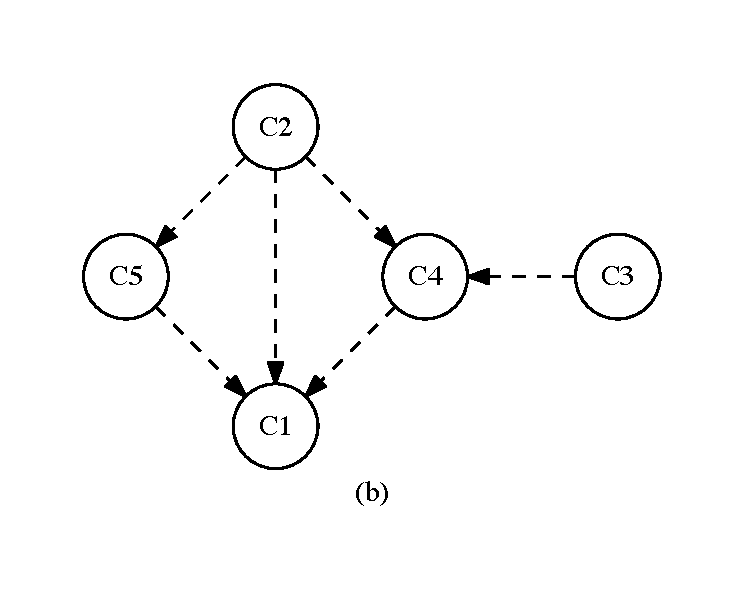
\includegraphics[width=0.57\columnwidth]{graphs/ccom.pdf}
%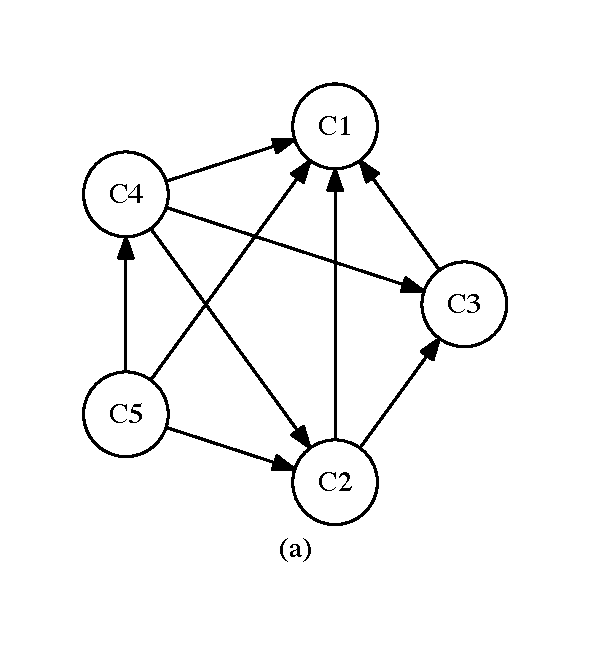
\includegraphics[width=0.40\columnwidth]{graphs/cart.pdf}
%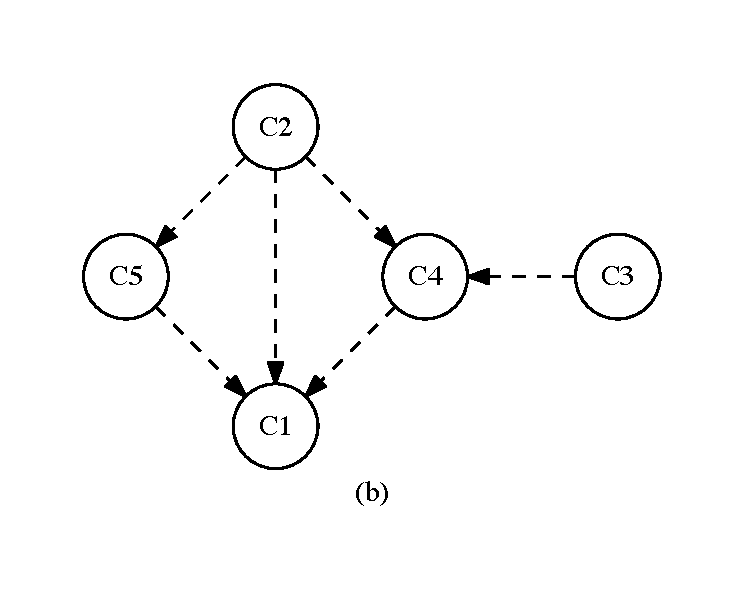
\includegraphics[width=0.35\columnwidth]{graphs/ccom.pdf}
%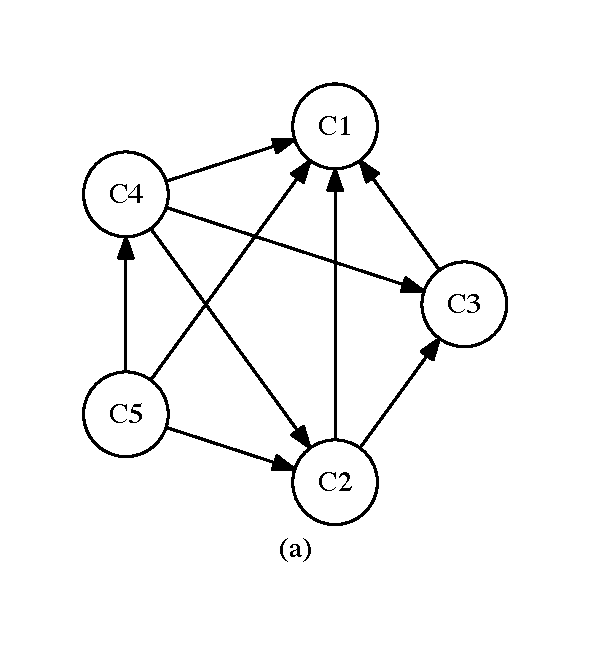
\includegraphics[width=0.35\columnwidth]{graphs/cart.pdf}
\includegraphics[width=0.35\columnwidth]{graphs/ccom.eps}
\includegraphics[width=0.35\columnwidth]{graphs/ccart.eps}
\vspace{-12pt}
\caption{Trend graphs for the CCC equivalence graph: (a) represent the comprehension analysis (RQ1) and (b) represent the artifact analysis (RQ2)}
\vspace{-12pt}
\label{fig:graphsforanalysis}
\end{figure}
%\begin{table}
%\centering
%\caption{Topological Sorting, with the left-most position being highest \label{topologicalResults}}
%\begin{footnotesize}
%\begin{tabular}{| l | l | l | l | l | l |} \hline
%				& CCC			& DBB 		& LBW & SNG & LIT \\ \hline
%U 			& C1 C5 C4 C2 C3 	& D3 D1 D2 	& L3 L2		& S2 S1		& T1 T2 T4 T3 \\
%C		& C1 C3 C2 C4 C5 	& D2 D1 D3	&  L3 L2 L1 	& S2 S1 S3 	& T1 T3 T2 T4 \\
%\hline
%\end{tabular}
%\end{footnotesize}
%\end{table}

\begin{table}
\centering
\caption{Topological Sorting, with the left-most position being highest (non-smelly) and the right-most being most smelly \label{topologicalResults} }
\vspace{-6pt}
\vspace{-2pt}
\begin{tabular}{| l | l | l |}  \hline
& Understandability & Community  \\ \hline
CCC & C1 C5 C3 C4 C2  &   C1 C3 C2 C4 C5  \\
DBB & D3 D1 D2  &   D2 D1 D3\\
 LBW & L3 L2	 &  L3 L2 L1 	\\
 SNG &  S2 S1 &  S2 S1 S3 \\
 LIT & T1 T3 T2 T4 & T1 T3 T2 T4 \\
\hline
\end{tabular}
\vspace{-6pt}
\vspace{-6pt}
\end{table}





%In the understandability graph, we represent a directed edge $\overrightarrow{C2C1}$ when match(C1) $>$ match(C2) \emph{and} compose(C1) $>$ compose(C2). When there is a conflict between match and compose, as is the case with T1 and T3 where match(T1) is higher but compose(T3) is higher, an undirected edge $\overline{T1T3}$ is used. When one metric has a tie, as is the case with composition in E9, we use the other metric to determine $\overrightarrow{C5C1}$. An example understandability graph for the CCC is shown in Figure~\ref{fig:graphsforanalysis}b. Nodes with few incoming edges are less understandable (or were not evaluated in our study), and nodes with more incoming edges were more understandable.
%\footnote{When there are confounded representations, as is the case with E8, E4, and E5 which all use transformations from the CCC and the LIT equivalence classes, we omit those from the understandability graph. This makes sense since all use a transformation between T1 and T4 strongly favoring T1. }

%\subsubsection{Topological Sorting}
\textbf{Topological Sorting:}
Once the two graphs are built for each equivalence class type, within each graph, we sort the nodes to identify a (preferably unique) total ordering on the nodes. This ordering represents preferences from the perspective of the comprehension or community standards metrics.
%we apply a modified version of Kahn's topological sorting algorithm to obtain a total ordering.
%The first modification is to remove all undirected edges since Kahn's operates over a directed graph.
%To begin, any disconnected nodes are added to the end of the topologically sorted list $L$.
%In Kahn's algorithm, all nodes without incoming edges are added to a set $S$, which represents the order in which nodes are explored in the graph. For each $n$ node in $S$, all edges from $n$ are removed and $n$ is added to a list $L$. If there exists a node $m$ that has no incoming edges, it is added to $S$. In the end, $L$ is a topologically sorted list.
%\begin{algorithm}
% \caption{Modified Topological Sort}\label{topological}
% \begin{algorithmic}[1]
%\State  $L \gets$ []
%\State $S \gets$ []
%\State Remove all undirected edges (creates a DAG) \label{removeundir}
%\State Add all disconnected nodes to $L$ and remove from graph. If there is more than one, mark the tie. \label{markTie1}
%\State Add all nodes with no incoming edges to $S$. If there is more than one, mark the tie. \label{addnoincomingtos}
%\While {$S$ is non-empty} \label{beginwhile}
%	\State remove a node $n$ from $S$ \label{setn}
%	\State add $n$ to $L$  \label{addntoL}
%	\For {node $m$ such that $e$ is an edge $\overrightarrow{nm}$}
%		\State remove $e$
%		\If{$m$ has no incoming edges}
%			\State add $m$ to $S$ \label{addToS}
%		\EndIf
%	\EndFor
%	\State If multiple nodes were added to $S$ in this iteration, mark the tie \label{markTie2}
%	\State remove $n$ from graph
%\EndWhile
%\State For all ties in $L$, use a tiebreaker.
%  \end{algorithmic}
%\end{algorithm}

For each node $n$, we compute the ratio of $in\_deg(n) / deg(n)$ where $in\_deg(n)$ is the number of incoming edges to $n$, and $deg(n)$ is the total edges touching~$n$. For example, in Figure~\ref{fig:graphsforanalysis}a, $in\_deg(C5) = 2$ and $deg(C5) = 5$.
The higher the ratio (that is, the more incoming edges indicating preference), the higher the node appears in the sorted list. For example, with node C1 in Figure~\ref{fig:graphsforanalysis}a, the ratio is $7 / 10$ since C1 is involved in ten total comparisons and is favored in seven. The ratio for node C2 is $1 / 5$ as C2 is involved in five comparisons, is preferred in one, is strictly not preferred in three, and has one with no preference, represented as an undirected edge.

One challenge with this (and any topological sorting approach, such as Kahn's algorithm), is that the total ordering is not necessarily unique and often multiple nodes have similar properties.
Thus, we mark ties in order to identify when a tiebreaker is needed.
% to enforce a total ordering on the nodes (though admittedly, it is not always unique).
%For example, on the understandability graph in Figure~\ref{fig:graphsforanalysis}, there is a tie between C3 and C2 since both have no incoming edges, so they are marked as a tie. Further, if C3 is added to $S$ first, when $n=C2$, both C5 and C4 are added to $S$, thus the tie between them is marked. In these cases, a tiebreaker is needed.
Breaking ties on the community standards graph involves choosing the representation that appears in a larger number of projects, as it is more widespread across the community.
Breaking ties in the understandability graph uses the RQ1 results. Based on Table~\ref{table:testedEdgesTable}, we compute the average metrics for each representation and select the winner.
%For example, C4 appears in E5, E12, and E13 with an overall average matching score of 0.81 and composition score of 24.3. C5 appears in E4 and E9 with an average matching of 0.87 and composition of 28.28. Thus, C5 is favored to C4 and appears higher in the sorting.

\subsection{Results}
The total orderings on nodes for each graph are shown in Table~\ref{topologicalResults}. For example, given the graphs in Figure~\ref{fig:graphsforanalysis}a and Figure~\ref{fig:graphsforanalysis}b, the topological sorts are {\tt C1 C5 C3 C4 C2} and {\tt C1 C3 C2 C4 C5}, respectively.



Considering both topological sorts, there is a clear winner in each equivalence class except DBB. 
%, with the exception of DBB.
%That is, the node sorted highest in the topological sorts for both the community standards and understandability analyses are
This is C1 for CCC, L3 for LBW, S2 for SNG, and T1 for LIT.
%While the least-smelly representation is relatively clear, the smelliest representation varies.
%After the top rank, the second rank varies depending on the metric, however, h
While L3 is the winner for the LBW group, we note that L2 appears in slightly more patterns.
DBB is different as the orderings are completely reversed depending on the analysis. %, so the community standards favor D2 and understandability favors D3.
Further study is needed on this, as well as LBW and SNG since not all nodes were considered in the understandability analysis.

These results can guide regex design.
For example, to match numbers from one to 999, there are (at least) three options: $A$~=~{\tt [1-9]|[1-9][0-9]|[1-9][0-9][0-9]}, $B$~=~{\tt [1-9][0-9]?[0-9]?}, and $C$~=~{\tt [1-9][0-9]\{0,2\}}.
$A$ contains representations \{C1, D3, S2\}, $B$ contains \{C1,~D2\}, and $C$ contains \{C1, D1\}. % D3 and S2, B contains C1 and D2, and C contains C1 and D1.
According to Table~\ref{topologicalResults}, the sorting in understandability is \texttt{A\textgreater C\textgreater B} since \texttt{D3\textgreater D1\textgreater D2}. However, what we usually see in source code are B and C but not A. The reason might be that the representation of A takes more time to type, or may have a longer runtime performance.
In another example, we prefer {\tt \$[0-9]*.[0-9][0-9]} to {\tt \$[0-9]*.[0-9]\{2\}} in order to match dollar amounts. This is because S2 in the former regex is preferred to S1 in the latter regex, for all metrics.
%

\subsection{Summary}
Having a consistent and clear winner is evidence of a preference with respect to community standards and understandability, and thus provides guidance for potential refactoring.
This positive result, that the most popular representation in the corpus is also the most understandable, makes sense as people may be more likely to understand things that are familiar or well documented.
